\documentclass[11pt,a5paper,landscape]{article}

\usepackage{main}
\usepackage{exercices}

% --------------------------------------------------
% Informations du document
% --------------------------------------------------
\renewcommand{\typedocument}{Exercices}
\renewcommand{\classe}{5e}
\renewcommand{\titre}{Exercices - Electricité}

\begin{document}
\begin{multicols*}{2}

% ----- Exercice 1 -----

\exercice{Schéma électrique}
Dessiner le schéma correspondant à ce circuit.
\begin{center}
    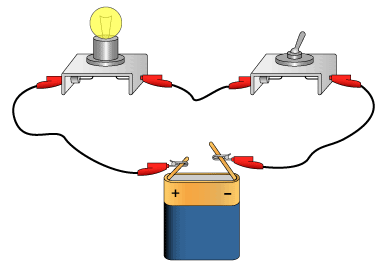
\includegraphics[width=3.3cm]{images/dessin circuit.png}    
\end{center}

% ----- Exercice 2 -----

\exercice{Circuits électriques}
Pour chacun des circuits suivants, indiquer si la lampe est allumée :

\begin{minipage}{2cm}
    a.
    
    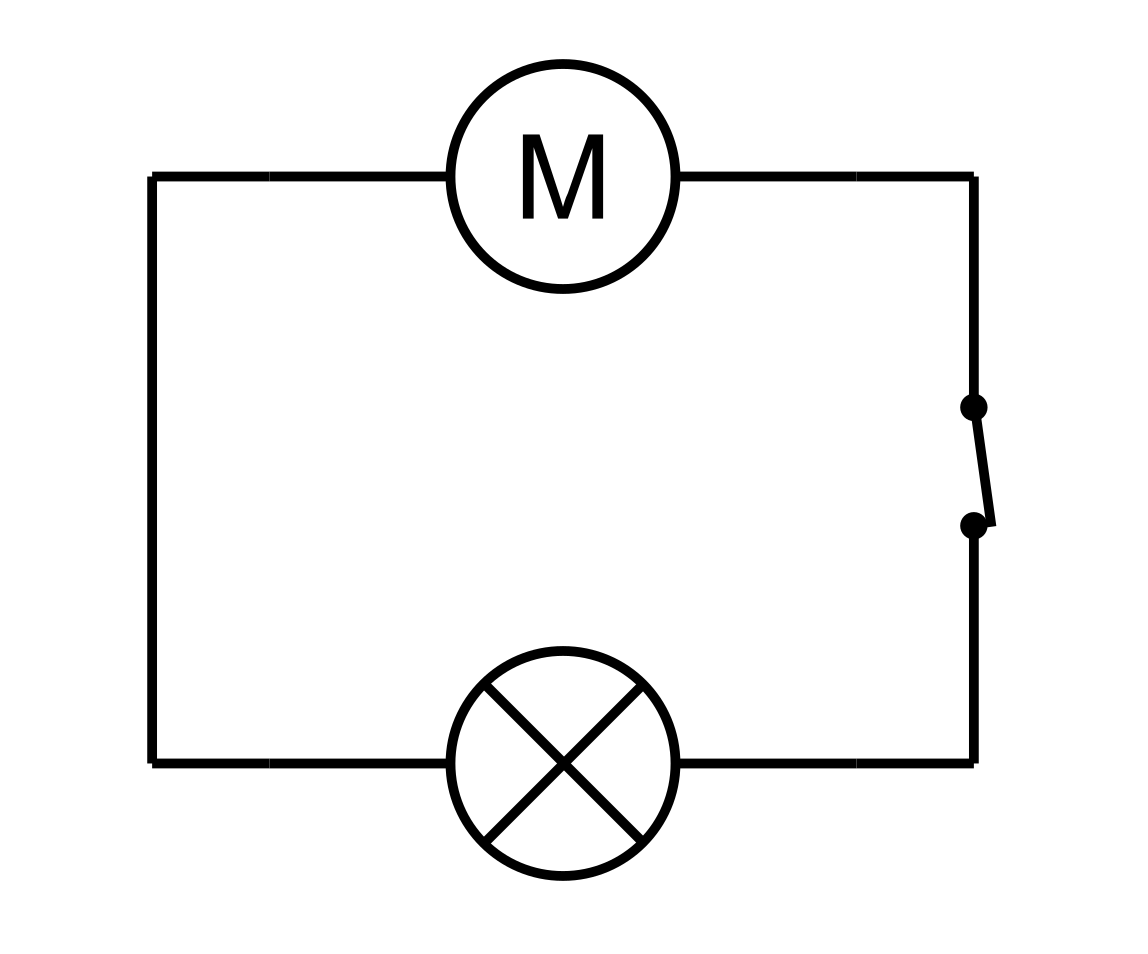
\includegraphics[width=2cm]{images/circuit a.png}
\end{minipage}
\hfill
\begin{minipage}{2cm}
    b. 
    
    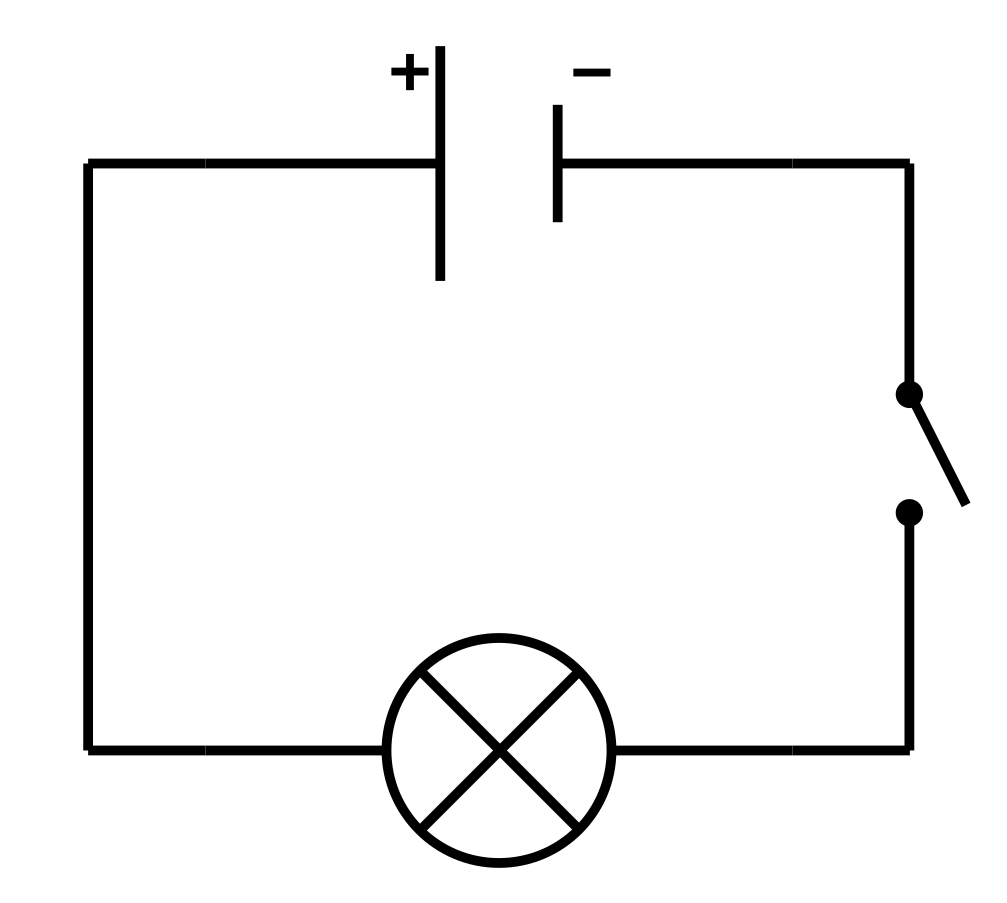
\includegraphics[width=2cm]{images/circuit b.png}
\end{minipage}
\hfill
\begin{minipage}{2cm}
    c.
    
    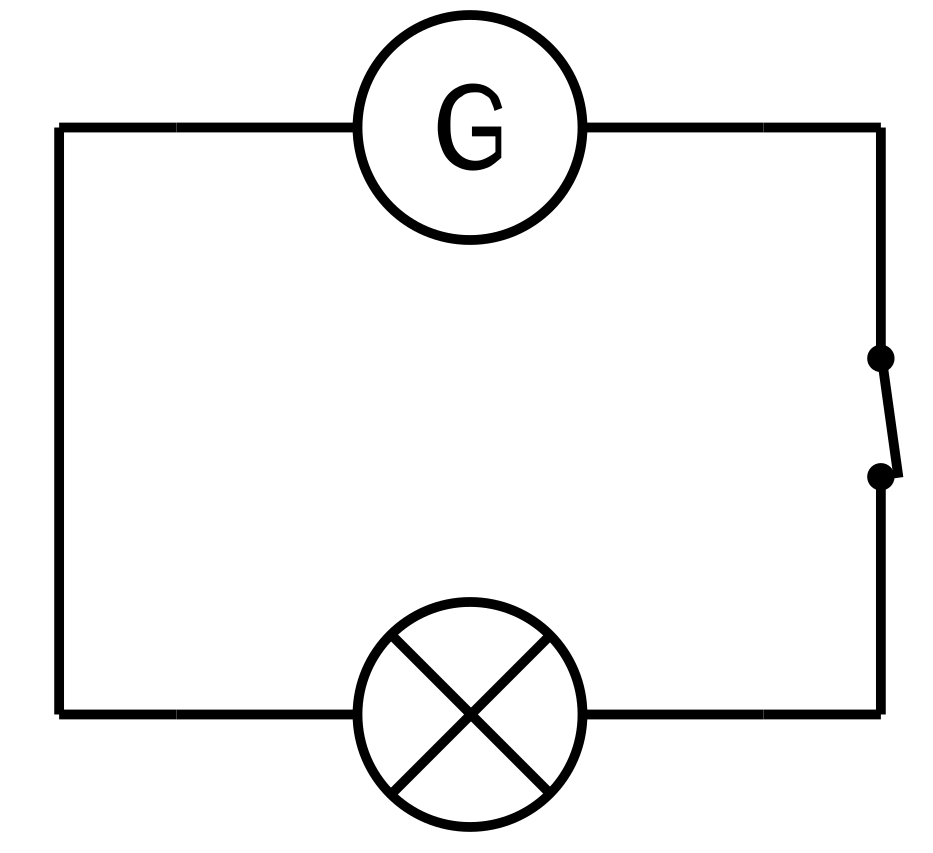
\includegraphics[width=1.7cm]{images/circuit c.png}
\end{minipage}
\hfill
\begin{minipage}{2cm}
    d.
    
    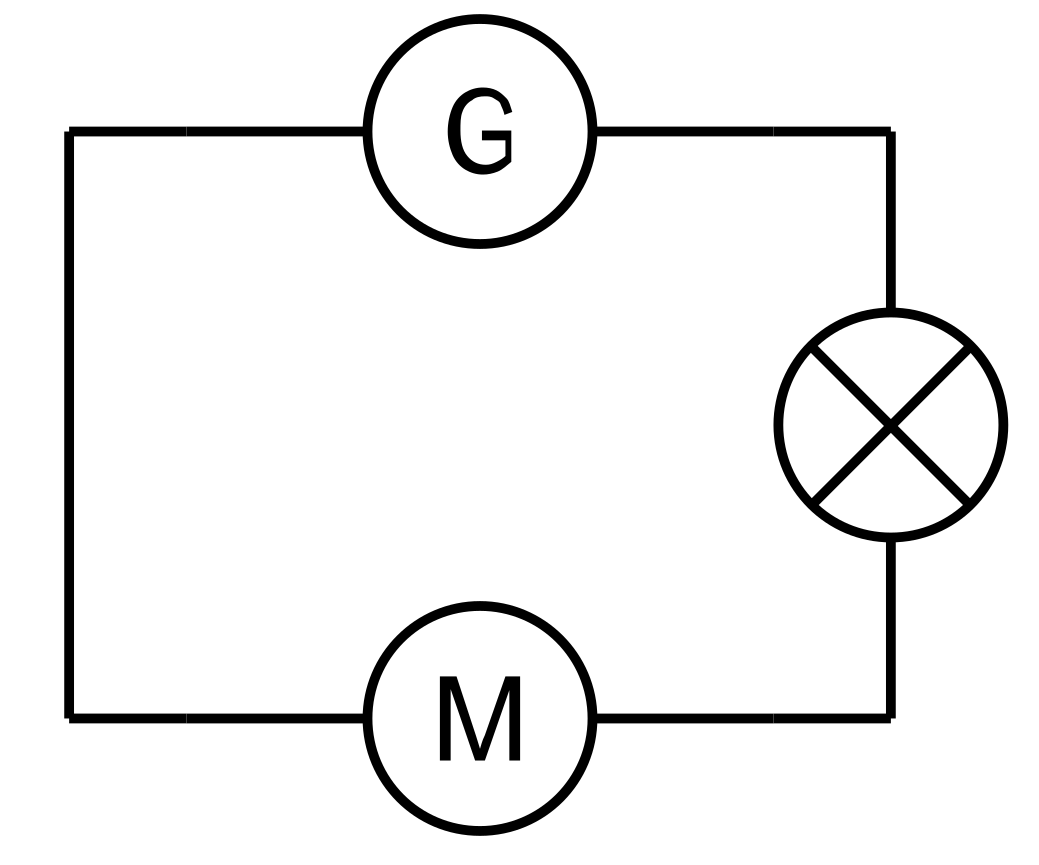
\includegraphics[width=2cm]{images/circuit d.png}
\end{minipage}


% ----- Exercice 3 -----

\exercice{Conducteurs ou isolants}

Lequel (ou lesquels) de ces objets est conducteur ?
\begin{enumerate}
    \item Une règle en plastique
    \item Une table en bois
    \item Une fourchette en métal
\end{enumerate}

\columnbreak

% ----- Exercice 4 -----

\exercice{}
Recopier et compléter les phrases suivantes :
\begin{enumerate}
    \item Si l’interrupteur est …, le circuit est fermé. Le … peut circuler.
    \item Si l’interrupteur est ouvert, le circuit est …
    \item Le courant circule de la borne … vers la borne … du générateur.
    %\item Pour empêcher les électrocutions, on protège les appareils électriques avec des matériaux …
\end{enumerate}

% ----- Exercice 5 -----

\exercice{}
Expliquer pourquoi les schémas électriques de Nicolas (à gauche) et Arthur (à droite) sont faux.

\begin{minipage}{4cm}    
    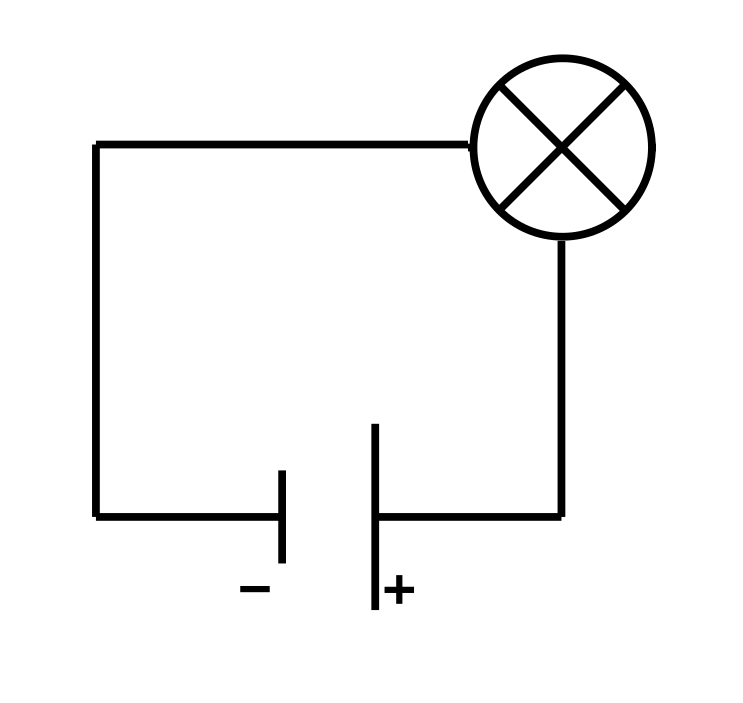
\includegraphics[width=2.4cm]{images/circuit nicolas.png} Nicolas
\end{minipage}
\begin{minipage}[c]{4cm}    
    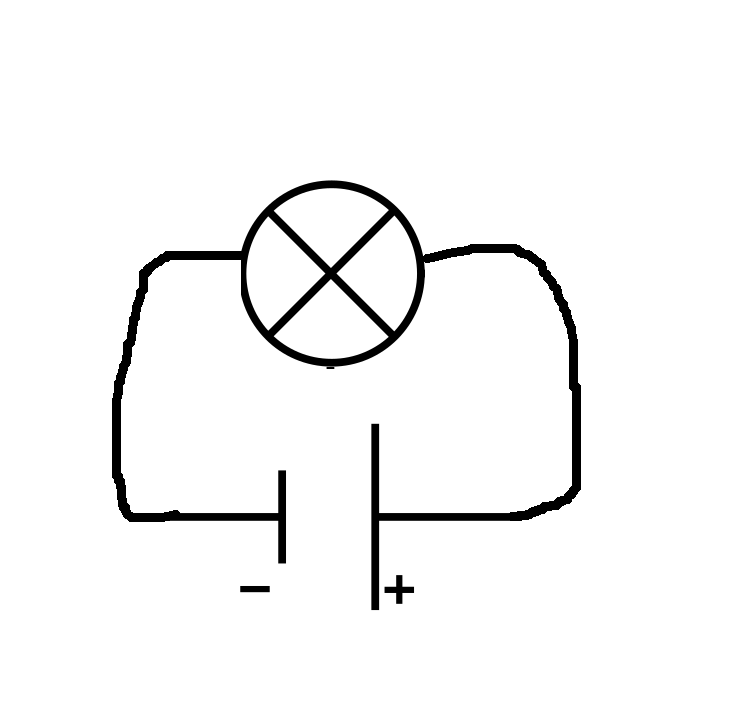
\includegraphics[width=2.4cm]{images/circuit arthur.png} Arthur
\end{minipage}

Pierre (à gauche) et Lia (à droite) ont schématisé le circuit électrique qu'ils ont réalisé. Est-ce que ces deux schémas correspondent au même montage ?

\begin{minipage}{5cm}    
    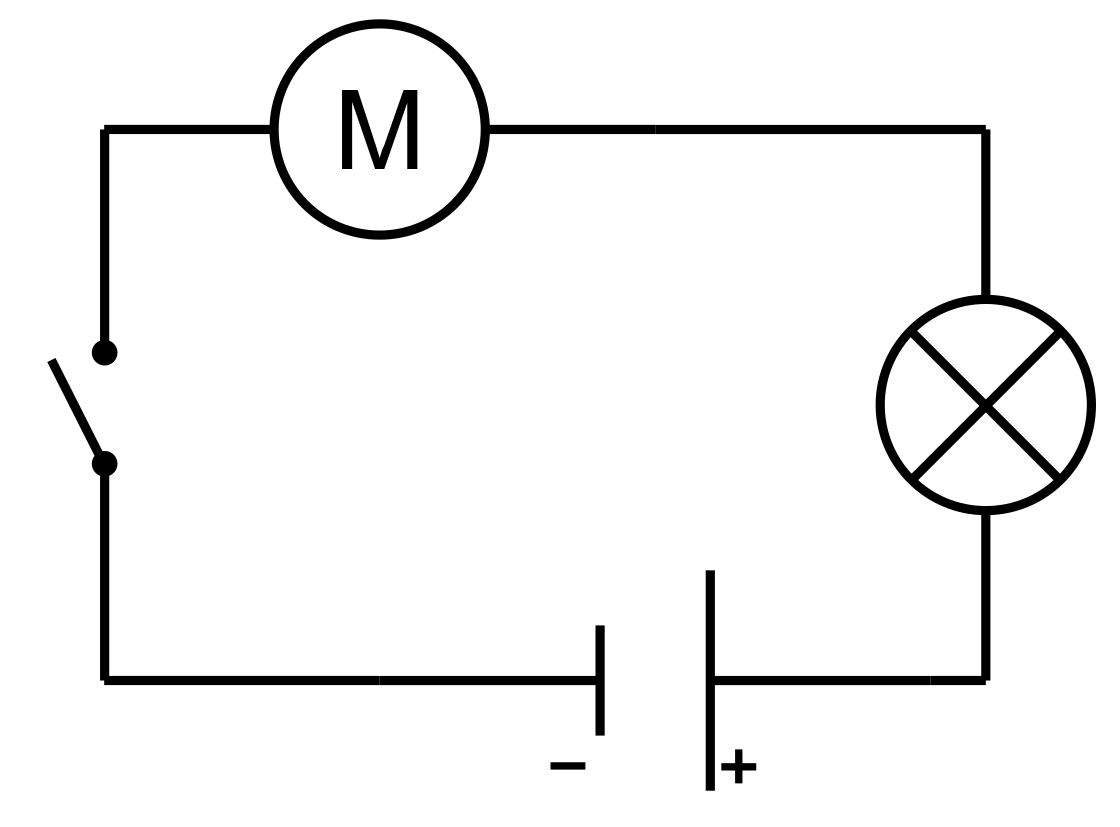
\includegraphics[width=2.4cm]{images/circuit pierre.png} Pierre
\end{minipage}
\hfill
\begin{minipage}{5cm}
    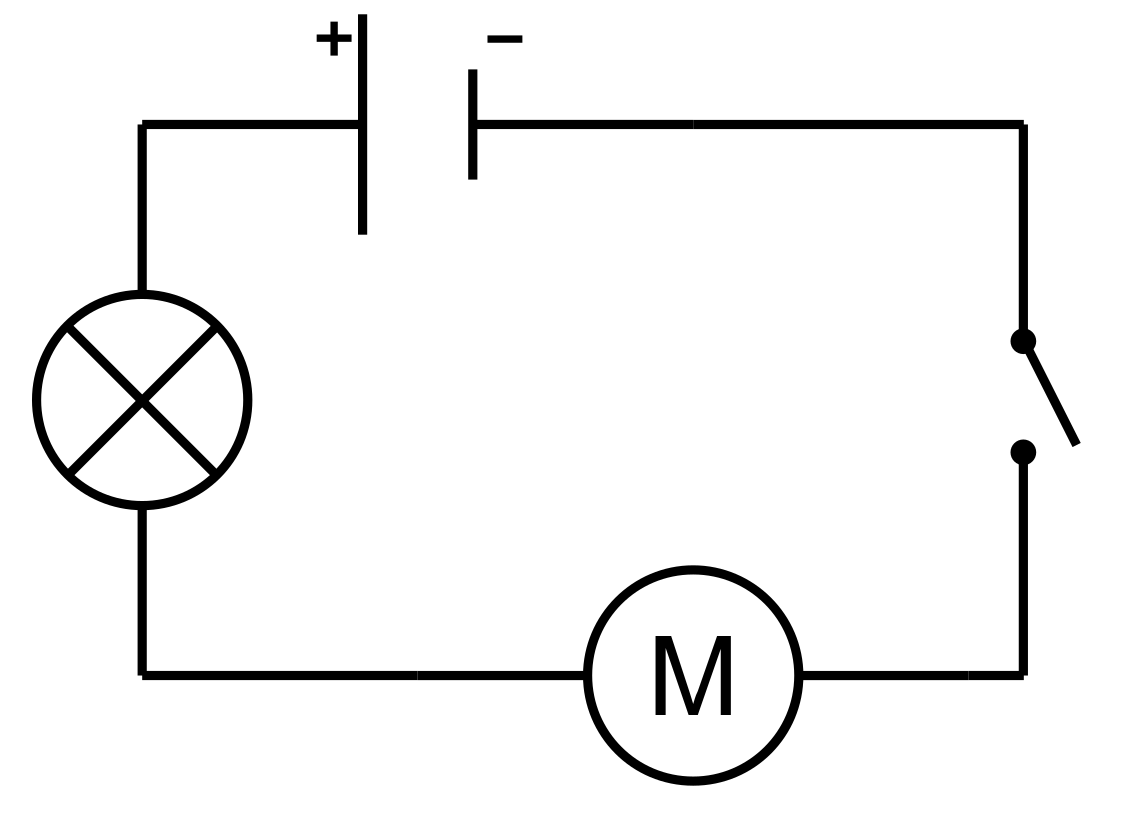
\includegraphics[width=2.4cm]{images/circuit lia.png} Lia
\end{minipage}


\end{multicols*}
\end{document}